%\clearpage
%\section{Experiments (Alt version; Restructured)}
\section{Experiments}
\label{sec:experiments}

%\sk{Potential restructure for section 3+4 (combined) below; relevant comments from section 3+4 still left inline} \\
% \sk{below is newer exp + discussion sections; relevant comments from old version kept inline; to use old experiment + discussion sections, uncomment in colm2026\_conference.tex file}

\def\changesize#1{\fontsize{#1}{10.5pt}\selectfont}
\begin{table*}[t]
\centering
\small
\fontsize{8.7pt}{10.5pt}\selectfont
    \renewcommand{\arraystretch}{1.18}
    \setlength{\tabcolsep}{2.7pt}
% \begin{tabular}{l@{\hspace{1.8pt}}c@{\hspace{2.3pt}}c@{\hspace{3pt}}c@{\hspace{2.3pt}}c@{\hspace{3pt}}c@{\hspace{2.3pt}}cc@{\hspace{2.3pt}}cc}
\begin{tabular}{l@{\hspace{1.6pt}}ccc@{\hspace{2pt}}c@{\hspace{2pt}}ccccc}
\toprule
 & \multicolumn{6}{c}{\textbf{Math}} & \multicolumn{2}{c}{\textbf{Code}} & \multirow{2}{*}{\textbf{Avg.}} \\
\cmidrule(lr){2-7} \cmidrule(lr){8-9}
 & {\changesize{8.3} AIME24} & {\changesize{8.3}AIME25} & {\changesize{8.3}HMMT25} & {\changesize{8.3}AMOBench} & {\changesize{8.3}OpenR1} & {\changesize{8.3}MATH} & {\changesize{8.3}Codeforces} & {\changesize{8.3}LCB} & \\
\midrule
\textbf{\qwen{}}           & 59.6 & 45.8 & 26.7 &  9.8 & 55.8 & 91.0 & 48.0 & 61.8 & 49.8 \\
SFT                        & 61.7 & 46.3 & 31.3 &  7.3 & 56.1 & 91.3 & 49.1 & 57.2 & 50.0 \\
RFT                        & 64.2 & 52.1 & 37.1 & \underline{11.3} & 59.3 & 91.9 & 50.9 & 68.0 & 54.3 \\
GRPO                       & 62.5 & 50.0 & 30.4 & 11.0 & \textbf{62.9} & \underline{93.5} & 52.2 & 62.6 & 53.1 \\
SDFT                       & 63.3 & 47.9 & 32.9 &  9.0 & 57.0 & 91.1 & 49.3 & 59.2 & 51.2 \\

% \rowcolor{lightyellow!50}
\textbf{\sft{}} (Ours)     & \underline{66.7} & \underline{59.2} & \underline{40.0} & \textbf{16.0} & 59.8 & 92.4 & \underline{52.7} & \underline{74.4} & \underline{57.6} \\

\rowcolor{lightblue!80}
\textbf{\ours{}} (Ours)    & \textbf{68.3} & \textbf{60.0} & \textbf{45.4} & \textbf{16.0} & \underline{60.4} & \textbf{93.6} & \textbf{56.1} & \textbf{82.6} & \textbf{60.3} \\
\midrule

\textbf{\olmo{}}           & 56.7            & 42.1            & 25.0            & 1.3            & 48.9            & 91.1            & 31.7            & 32.4            & 41.1            \\
SFT                        & 51.3            & 43.8            & 30.4            & 1.3            & 48.5            & 91.4            & 31.7            & 41.0            & 42.4            \\
RFT                        & 56.7            & 48.3            & 35.8            & 2.3            & 50.9            & 91.4            & 39.2            & 49.4            & 46.7            \\
GRPO                       & 54.6            & 43.8            & 25.8            & \underline{4.8} & \textbf{56.9}   & 91.8            & 37.1            & 43.6            & 44.8            \\
SDFT                       & 52.9            & 45.0            & 32.1            & 1.3            & 49.0            & 91.2            & 33.5            & 42.3            & 43.4            \\
\textbf{\sft{}} (Ours)     & \underline{59.2} & \underline{52.9} & \underline{39.6} & 3.5            & 52.4            & \underline{92.3} & \underline{42.8} & \textbf{59.6}   & \underline{50.3} \\
\rowcolor{lightblue!80}
\textbf{\ours{}} (Ours)    & \textbf{61.7}   & \textbf{53.8}   & \textbf{40.4}   & \textbf{5.5}   & \underline{55.3} & \textbf{94.0}   & \textbf{43.5}   & \underline{57.8} & \textbf{51.5}   \\
\bottomrule
\end{tabular}
\caption{\textbf{Performance comparison of \ours{} and \sft{} (Self-Revision Training, Phase~1) against baseline post-training methods} on math and code reasoning benchmarks, reported as avg@8. Across both \qwen{} and \olmo{}, \sft{} and especially \ours{} achieve the strongest overall results; “LCB” denotes LiveCodeBench. All methods are compute equalized (see Appendix \ref{app:compare-budget} for more details).}
\vspace{-10pt}
\label{tab:main_results}
\end{table*}

\subsection{Experimental Setup}
\label{sec:setup}

\looseness-1\textbf{Models.} We use \qwen{} \citep{yang2025qwen3technicalreport} and \olmo{} \citep{olmo2025olmo3} as base models. All sampling uses temperature 0.7 with a 16K token limit during training and a 32K limit at evaluation. We report avg@8 throughout.

\looseness-1\textbf{Datasets.} We train on two domains separately: (1)~\textbf{OpenR1-Math} \citep{openr1}, from which we select 15K competition- and olympiad-level problems with verified solutions, and (2)~\textbf{Codeforces} \citep{penedo2025codeforces}, from which we select 7.5K samples from the cpp (\texttt{solutions}) subset and 7.5K from the Python (\texttt{solutions\_py}) subset. We include more details on training data curation in Appendix \ref{app:training-data}.

% \sk{also include sampling budget + more details for revision sper question num questions, etc}

\looseness-1\textbf{Evaluation. } We evaluate on eight benchmarks in math and code domains: competition math (AIME24 \citep{aime24}, AIME25 \citep{aime25}, HMMT25 \citep{hmmt_2025}, MATH \citep{hendrycks2021measuringmathematicalproblemsolving}), olympiad math (AMOBench~\citep{an2025amobenchlargelanguagemodels} and OpenR1-Math \citep{openr1}), and competitive programming (Codeforces \citep{penedo2025codeforces} and LiveCodeBench \citep{jain2024livecodebenchholisticcontaminationfree}). For the two in-distribution datasets we hold out 500 test questions each.


\looseness-1All baselines train on the same 15K questions: (1)~\textbf{SFT} on high-quality demonstrations from DeepSeek-R1~\citep{Guo_2025}, (2)~\textbf{RFT}, rejection fine-tuning on correct self-generated traces \citep{yuan2023scalingrelationshiplearningmathematical}, (3)~\textbf{GRPO} with binary correctness reward \citep{grpo} \footnote{\looseness-1We use DAPO (\citet{yu2025dapo}), an improved and commonly used variant of GRPO.}, and (4)~\textbf{SDFT}, on-policy self-distillation with the model conditioned on high-quality demonstrations as its own teacher \citep{zhao2026selfdistilledreasoneronpolicyselfdistillation, shenfeld2026selfdistillationenablescontinuallearning}. 
% \danqi{Why do you call it OPSD, not SDFT? Does it always have access to CoT from DeepSeek-R1? You probably need a baseline that the teacher has access to only input and answer?}
We attach a detailed comparison of sampling budgets across \ours{} and baseline methods in Appendix \ref{app:compare-budget}, and training hyperparameters in Appendix \ref{app:hyperparameters}.

 
%\subsection{Self-Revision Training Performs Stronger than Training on Expert Solutions or Filtered Self-Generations}
\subsection{SRT Outperforms Training on Expert Solutions or Filtered Self-Generations}
%\subsection{\ours{} improves the }
\label{sec:srt-results}

%\textbf{Self-Revision Training Teaches Inference-Time Error Correction Better.} 
%\ap{take a pass; maybe shorten}
%One might expect that expert solutions (SFT) or filtered correct self-generations (RFT) would provide a strong offline training signal. 

\looseness-1We first compare \sft{} against training on high-quality demonstrations (SFT) and filtered correct self-generations (RFT) (Table~\ref{tab:main_results}). Trained on only 6K self-revision responses, \sft{} improves average accuracy by 7.8\% on \qwen{} and 9.2\% on \olmo{}, substantially outperforming both SFT and RFT trained on 15K examples. The baselines fail for different reasons: SFT on DeepSeek-R1 responses degrades \qwen{} on benchmarks such as AMOBench and LiveCodeBench, while RFT shows minimal gains on harder tasks such as AMOBench.

\looseness-1\sft{} is effective because it supervises error correction: each example pairs an on-policy incorrect attempt with a self-corrected revision; we find that correctness filtering of revision traces is important (Appendix \ref{app:countdown}). Unlike RFT, which removes incorrect reasoning entirely, \sft{} preserves the failed attempt as context, allowing the model to learn from its own mistakes. This structure yields especially strong gains on harder benchmarks such as AIME25, HMMT25, and LiveCodeBench.

% \looseness-1We first compare performance of \sft{} with training on an high-quality demonstrations (SFT) or filtered correct self-generations (RFT) (Table~\ref{tab:main_results}). \sft{}, trained on only 6K self-revision responses, improves average accuracy by 7.8\% on \qwen{} and 9.2\% on \olmo{}, significantly surpassing both SFT and RFT training on 15K examples. 
% The two baselines each fail for separate reasons: SFT on DeepSeek-R1 responses leads to degradation in the performance of \qwen{} on benchmarks such as AMOBench and LiveCodeBench. RFT  shows minimal improvement on hard tasks such as AMOBench.



% \looseness-1\sft{}’s effectiveness comes from supervising the process of correcting an incorrect response, with instances containing an on-policy incorrect attempt paired with a self-corrected attempt; we find that correctness filtering of revision traces is important (Appendix \ref{app:countdown}). While SRT retains the incorrect attempt as context, RFT filters out all incorrect reasoning, so the model never sees its own failure.
% This error-correction structure helps \sft{} achieve substantial gains on harder benchmarks such as AIME25, HMMT25, and LiveCodeBench.


% but stalls where the base model rarely solves problems: AMOBench gains only 1.5\% (\qwen{}) and 1.0\% (\olmo{}) under RFT, versus 6.2\% and 2.2\% under \sft{}. 
% \sk{might need more details since we say baselines are trained on same 15k examples and experiments are compute controlled}
% (AIME25 +13.4\%, HMMT25 +13.3\%, LiveCodeBench +12.6\% for \qwen{})
%, despite training only on OpenR1-Math and Codeforces.


\begin{wrapfigure}{r}{0.35\textwidth}
    \vspace{-13pt}
  \centering
  \captionsetup{font=footnotesize}
  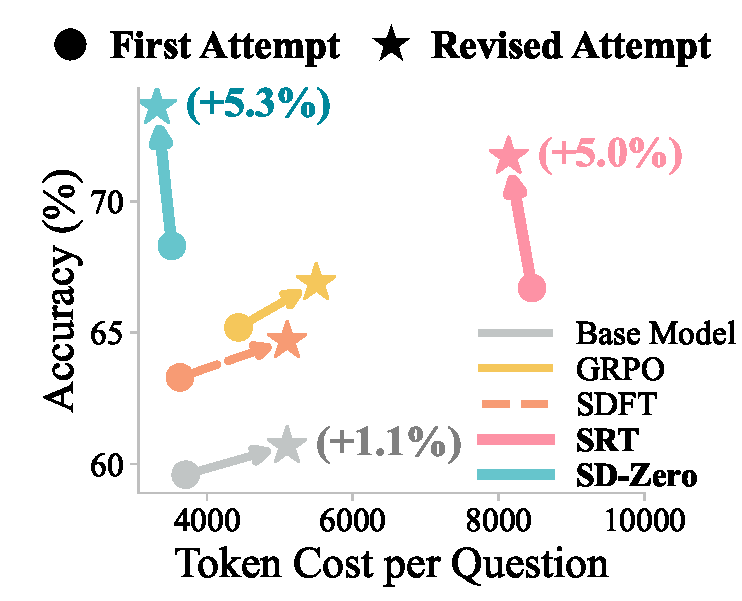
\includegraphics[
    width=0.35\textwidth,
    trim=0.7cm 0.1cm 0.1cm 0.4cm,
    clip
  ]{figures/trade_off_plot.pdf}
  \vspace{-15pt}
  \caption{\textbf{Comparison of outcome-conditioned self-revision capability} on AIME24, \qwen{}. \sft{} unlocks self-revision behaviors, while final \ours{} model preserves this advantage while improving token efficiency.}
  \label{fig:self-revision}
  \vspace{-5pt}
\end{wrapfigure}
\looseness-1\textbf{\sft{} Significantly Boosts Self-Revision Capability.}
To measure directly, we run a Generate-then-Revise evaluation on 1K AIME24 questions using \qwen{}: (1) \textit{First Attempt}: sample one response per question, (2) \textit{Revised Attempt}: prompt the model to generate a revision conditioned on the first attempt and its binary correctness reward. As shown in Figure~\ref{fig:self-revision} (detailed statistics in \Cref{tab:revision-token-tradeoff}), while the base model gains only $1.1\%$ from revision, \sft{} gains $+5.0\%$, indicating that the \sft{} model has learned to use outcome reward to correct its first attempt rather than simply resampling a new attempt. 
Notably, the revision responses produced by \sft{} are, on average, even shorter than the model’s first attempts, suggesting more targeted and proactive reasoning during revision; in contrast, revisions from the base model tend to be longer and likely more redundant. More interestingly, the self-revision capability of the model improves further after the \opsd{} phase. This observation is central to the self-evolving nature of \ours{}, which we discuss further in \Cref{sec:self-evolution}.

%This self-revision capability emerges in the \sft{} phase and is preserved through \ours{}, which further improves overall performance with less token cost.
% With \sft{} phase explicitly unlocking self-revision behaviors, the \ours{} phase preserves this gain while further improving overall performance, showing that this learned revision behavior can be transferred to later training stages.
% , using fewer tokens for the revisions than for the first attempt. This suggests that \sft{}
% The contrast is sharp: baselines produce longer, apparently redundant revisions, while the \sft{} model makes targeted corrections.


\subsection{Self-Distillation Distills Revision into Token-Efficient Generation}
\label{sec:distillation-results}

% After \sft{}, the model tends to produce two attempts within a single response, the second revising the first. This is effective but expensive. 
\looseness-1After \sft{}, the model as a generator tends to produce longer responses (as shown in \Cref{fig:self-revision}) with significantly more self-revision behaviors.
\opsd{} phase distills the self-revision behavior of the model back into more proactive responses of the generator.
%Concretely, the student generates a response $y_\text{init}$ given question $x$. The teacher sees $(x, y_\text{init}, P_r)$, the same response together with the binary reward of that attempt, and provides token-level supervision via KL divergence.


\looseness-1\textbf{\opsd{} Enables Stronger, Token-Efficient Generations.}
\Cref{tab:main_results} shows that \opsd{} phase adds $2.7\%$ on \qwen{} and $1.2\%$ on \olmo{} beyond \sft{}, for total gains of $+10.5\%$ and $+10.4\%$ over the base models. For \qwen{}, the gains concentrate on code benchmarks and HMMT25. For \olmo{}, the \opsd{} phase mainly improves on math benchmarks such as AIME24 and AMOBench. We also report pass@8 results in \Cref{tab:pass8_results}. Interestingly, pass@8 improves substantially as well, suggesting that \ours{} does not merely sharpen the output distribution, a behavior often associated with RL-based methods such as GRPO \citep{yue2025does}.


%Pass@8 performance (see \Cref{tab:pass8_results}) also shows a consistent improvement, which suggests that our method is not merely sharpening its output distribution, a phenomenon generally observed with RL based algorithms

%, indicating that our method is 
%not merely sharpening the output distribution, but genuinely guiding the model’s exploration to be more well-directed.
% LiveCodeBench actually drops 1.8\%. 
% Phase~2 appears more helpful for code than for math.\yh{benchmark gains}

\looseness-1Furthermore, as shown in \Cref{fig:self-revision},  \ours{} model generates only half as many tokens as \sft{} trained model and fewer tokens than all baselines, while achieving the strongest overall performance. We provide a deeper analysis  in \Cref{sec:behavioral_analysis}, where we show that distilling from the reviser helps the generator to produce more proactive and efficient responses.
% As such, we can view \ours{} as a process that distills the self-revision of the model into improved model's generation attempts, while actively reducing token cost.

% Its revised attempt requires even fewer tokens, while continuing to gain $5.3\%$.

\looseness-1\textbf{Comparison to \sft{}.} Since most of the performance gains in \ours{} arise during the \sft{} phase, one may question the importance of \opsd{}. We argue that \opsd{} is nevertheless a critical component of the \ours{} pipeline for two reasons. First, \opsd{} reduces response length at inference by at least $2\times$, substantially improving inference-time efficiency (\Cref{fig:self-revision}). Second, \opsd{} is highly sample-efficient during training. Constructing the \sft{} dataset requires collecting multiple sampled responses per question in order to obtain successful revisions, whereas \opsd{} requires only a single response per question and uses the reviser’s token-level feedback to provide dense supervision. We provide a detailed sample budget analysis in Appendix \ref{app:compare-budget}.

%\sk{prev sentence incomplete?}
%\yh{1.less token,2.sample efficient (mention rollout budget)} 

\looseness-1\textbf{Comparison to GRPO and SDFT.}  \ours{} outperforms by at least $4.8\%$ on average across benchmarks. These comparisons are made under a matched generation budget, where all methods use the same set of questions and are normalized by the number of model-generated responses in their respective pipelines.

% \begin{wraptable}{r}{0.34\textwidth}
% \vspace{-10pt}
% \centering
% \def\arraystretch{1.1}
% \setlength{\tabcolsep}{4pt}
% \fontsize{8pt}{8.5pt}\selectfont
% \begin{tabular}{lc}
% \toprule
% Method & \textbf{Avg.} \\
% \midrule
% Base model                & 48.1 \\
% $+$SDFT                      & 49.7 \\
% $+$SDFT (final answers only) & 49.5 \\
% $+$\ours{}            & \textbf{57.3} \\
% \bottomrule
% \end{tabular}
% \captionsetup{font=footnotesize}
% \caption{}
% \label{tab:sdft_final_answers_avg}
% \vspace{-0.8em}
% \end{wraptable}

\looseness-1We emphasize that this improvement is substantial for two reasons. First, unlike SDFT, that require gold solutions for each problem, \ours{} requires only a scalar reward on the model’s first attempt. In \Cref{tab:sdft_final_answers}, we show that SDFT performs much worse when given access only to the final answer but not the gold solutions. 
Second, unlike GRPO, whose training requires a group of sampled responses per question, the \opsd{} phase of \ours{} uses only a single response per question, substantially reducing generation cost.
While we note that GRPO may benefit from additional training epochs, our comparison is under a matched single-epoch budget, where \ours{} achieves stronger performance with comparable total sample cost (see Appendix \ref{app:compare-budget} for detailed budget analysis).

%\textbf{More concretely, \ours{} returns the best yield in performance per the number of generated responses from a given model, without requiring excess to an external teacher.} 



\begin{tcolorbox}[
  colback=lightblue!50,
  colframe=vividblue,
  boxrule=0.8pt,
  arc=2pt,
  left=6pt,
  right=6pt,
  top=4pt,
  bottom=4pt
]
\looseness-1 \textbf{Takeaway:} \ours{} offers the best performance per model generations among the compared methods, while requiring neither an external teacher nor high-quality demonstrations.
\end{tcolorbox}

% \begin{center}
% \fbox{
% \parbox{0.95\linewidth}{
% \textbf{Takeaway:} \ours{} offers the best performance per generation cost among the compared methods, while requiring no external teacher or gold solutions.
% }}
% \end{center}
% \begin{center}
% \fbox{
% \parbox{0.95\linewidth}{
% \textbf{Takeaway:} \ours{} offers the best performance per generation cost among the compared methods, while requiring no external teacher or gold solutions.
% }}
% \end{center}



% \ap{restructure}
% The central advantage over SDFT is that \ours{}'s teacher requires no expert-curated reasoning traces, making \ours{} applicable wherever a verifier exists. Compared to GRPO, \ours{}'s \opsd{} phase requires only one rollout per sample rather than a group, thereby significantly reducing sampling costs. 
% In our experiments, we run all baselines with the same total generation budget as \ours{} across Phases 1 and 2, and in fact give slightly more budget to baselines (see \Cref{app:compare-budget}). Despite this, \ours{} still outperforms both GRPO and SDFT by at least $4.8\%$ \yh{check stats}. Moreover, our \opsd{} phase is substantially more sample-efficient than the \sft{} phase. As training proceeds, \ours{} should eventually lead to faster gains for the same number of generations.

% however, Phase~1 (\sft{}) also incurs a sampling cost during data collection, so the fair comparison is total sampling budget across both phases versus GRPO's group size multiplied by training steps.

% \yh{comparison with GRPO and SDFT performance on complete benchmarks.}

% \sk{last point is probably generally true for SDFT-style method; maybe correct comparison is number of rollouts for \sft{} + self-distillation vs GRPO?}


% The per-benchmark gains are uneven. 
% we suspect code revision has more structured corrective patterns that distill more cleanly, but we have not confirmed this.
%\sk{It seems that Phase 2 is more helpful for code than for math (based on comparing the delta from \sft{} to self-distillation). Maybe that could be a discussion point? We can also brainstorm a plausible explanation.}

% \sk{should we also report pass@1 and pass@16 (maybe in the appendix)? That would allow us to comment on sharpening behavior (via pass@1) and whether \sft{}+self-distillation raises the ``ceiling'' of what the model can learn.}


\begin{figure}[t]
    \centering
    % \begin{subfigure}[t]{0.25\textwidth}
    %     \centering
    %     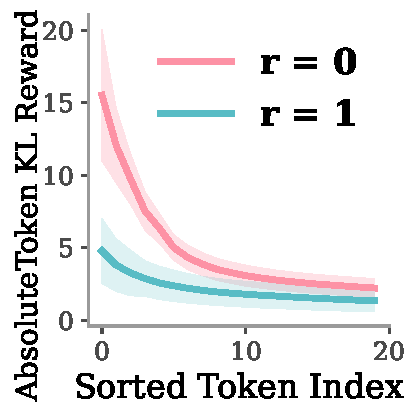
\includegraphics[width=\linewidth]{figures/token_rewards_correct_vs_incorrect.pdf}
    %     \captionsetup{width=0.9\linewidth}
    %     \caption{}
    %     \label{fig:credit-assignment-a}
    % \end{subfigure}
    % \hfill
    % \begin{subfigure}[t]{0.73\textwidth}
    %     \centering
    %     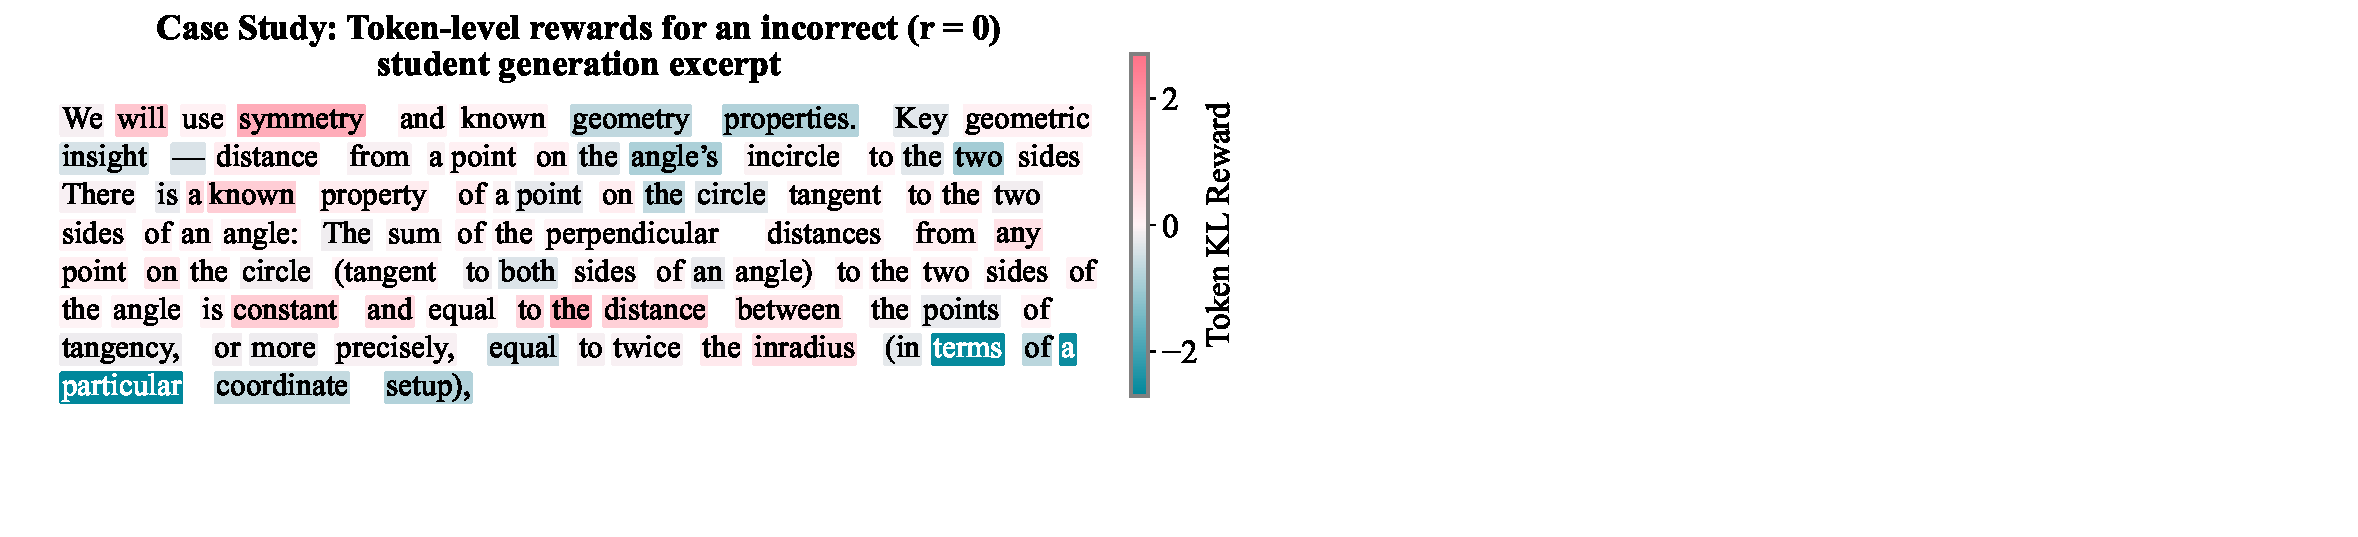
\includegraphics[
    %         width=\linewidth,
    %         trim=0.5cm 2cm 19cm 0cm,
    %         clip
    %     ]{figures/sample_9013_excerpt_token_reward_heatmap.pdf}
    %     \captionsetup{width=0.9\linewidth}
    %     \caption{}
    %     \label{fig:credit-assignment-b}
    % \end{subfigure}
    \captionsetup{font=small}
    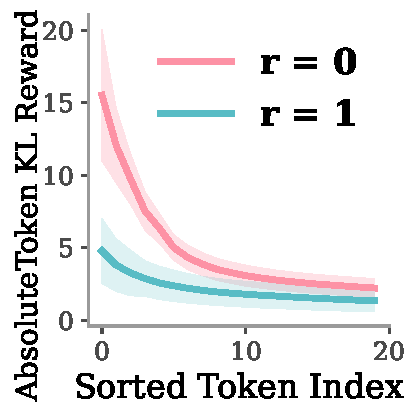
\includegraphics[width=0.25\textwidth]{figures/token_rewards_correct_vs_incorrect.pdf}
    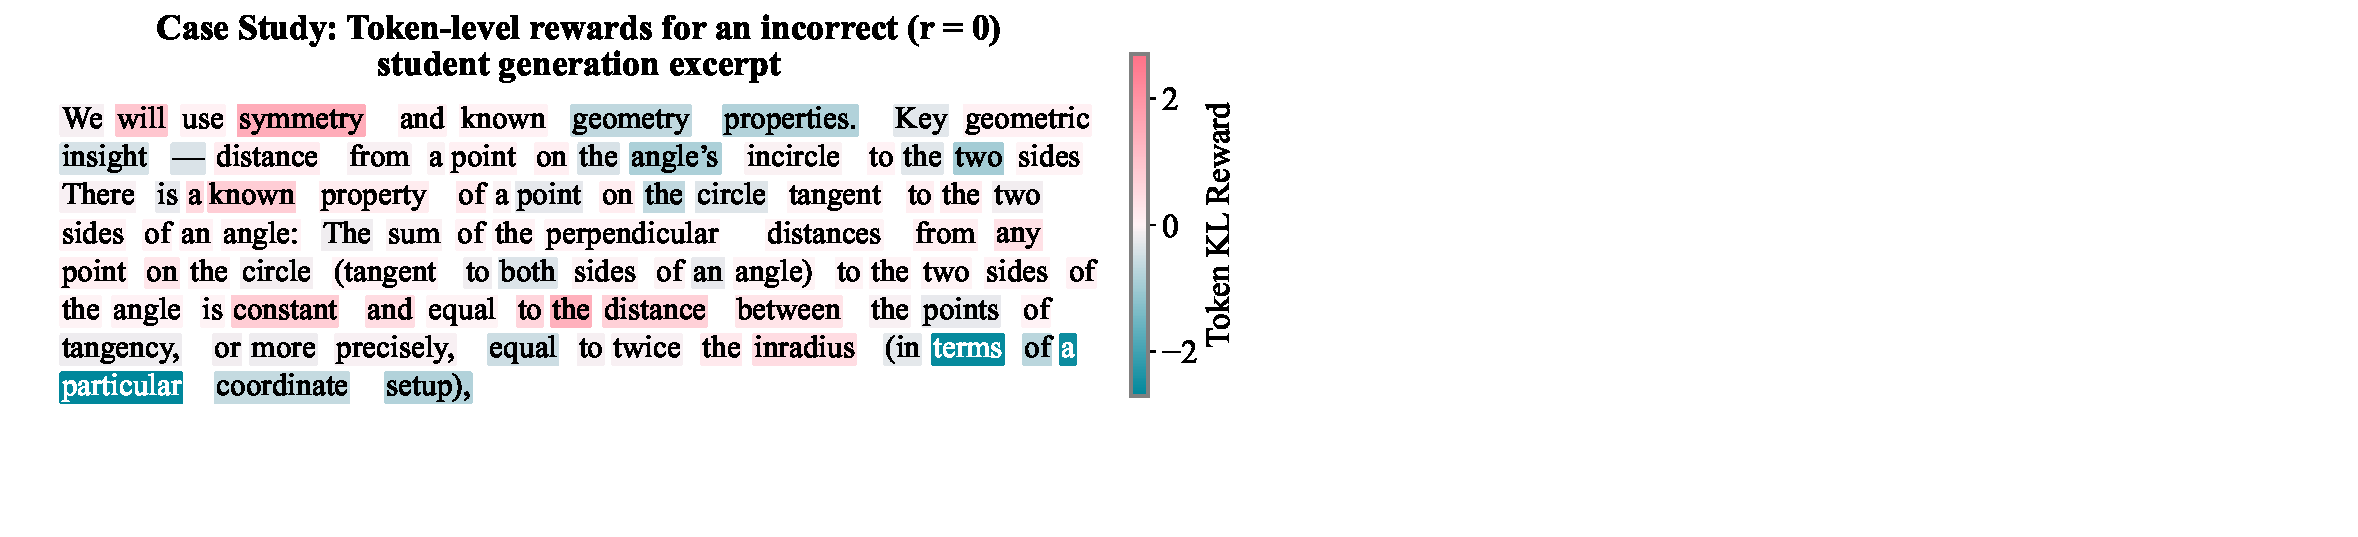
\includegraphics[
            width=0.73\textwidth,
            trim=0.5cm 2cm 19cm 0cm,
            clip
        ]{figures/sample_9013_excerpt_token_reward_heatmap.pdf}
    \caption{\looseness-1\textbf{Reviser converts binary outcome reward into dense token-level reward.}
\textbf{Left:} Comparison of token-level KL reward distributions for correct (\(\mathbf{r=1}\)) and incorrect (\(\mathbf{r=0}\)) student generations.
Incorrect trajectories concentrate larger rewards on a small number of tokens, whereas correct trajectories receive a flatter reward distribution that mainly preserves the response.
\textbf{Right:} Visualization of token-level KL rewards for an incorrect student generation (\(\mathbf{r=0}\)).
The teacher policy converts binary reward \(r=0\) to dense rewards that localize mistake-relevant tokens and guide targeted correction. 
}
    \vspace{-10pt}
    \label{fig:credit-assignment}
\end{figure}


\subsection{Iterative Self-Evolution: Teacher Synchronization Enables Continued Gains}
\label{sec:self-evolution}




\begin{wrapfigure}{r}{0.34\textwidth}
  \vspace{-10pt}
  \centering
  \captionsetup{font=footnotesize}
  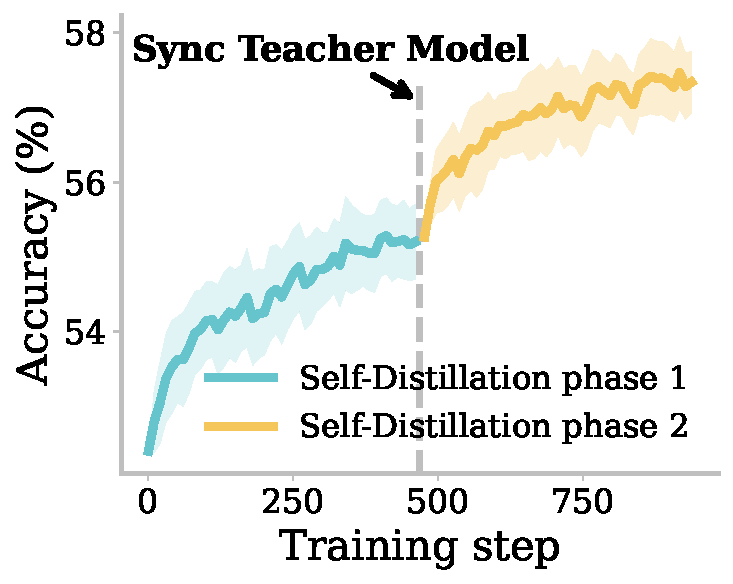
\includegraphics[
    width=0.32\textwidth,
    trim=0.2cm 0cm 0.3cm 0.3cm,
    clip
  ]{figures/evolution_plot.pdf}
  \vspace{-5pt}
  \caption{\textbf{Self-evolved reasoning through teacher synchronization in \ours{}.} \ours{} can iteratively improve the model by reusing its own learned self-revision behavior as supervision.}
  \label{fig:evolution}
  \vspace{-20pt}
\end{wrapfigure}


\looseness-1In \ours{} setup, the teacher is fixed as the \sft{} model throughout Phase~2. Performance eventually plateaus because the supervision signal is bounded by a stale teacher. But \opsd{} phase also improves the model's revision capability: the \ours{} model achieves a 5.3\% revision gain on the Generate-then-Revise evaluation, comparable to \sft{}'s 5.0\% (\Cref{fig:self-revision}). 
The improved student can therefore serve as a stronger teacher, enabling what we call \textbf{\emph{iterative self-evolution}}. The capability to revise answers is distilled back into generation, and regular teacher synchronization allows the loop to sustain.

\looseness-1We test this by synchronizing the teacher with the trained student after one epoch and continuing training. Figure~\ref{fig:evolution} shows the result on OpenR1-Math (\qwen{}): the first \opsd{} phase saturates around step 400; after teacher synchronization, a second phase yields at least 3 additional percentage points without signs of saturation. Once primed by \sft{}, the model can continue to self-evolve through iterated teacher synchronization, requiring only the initial attempt and corresponding binary reward in the teacher's context.
